\documentclass[a4paper,12pt,russian]{article} %draft
\usepackage[T2A]{fontenc}% Поддержка русских букв


% XeTeX packages
\usepackage[cm-default]{fontspec} % or install lmodern and remove cm-default opt
\usepackage{xunicode} % some extra unicode support
\usepackage{xltxtra} % \XeLaTeX macro


\tolerance=1000
\emergencystretch=0.74cm
\usepackage{indentfirst} %делать отступ в начале параграфа

\usepackage[pdfborder = {0 0 0}]{hyperref} %гиперссылки в документе.

\usepackage[utf8]{inputenc}	% кодировка текста
\usepackage[russian]{babel}	% руссификация по Бабелю
\usepackage{graphics}

\usepackage[clean,pdf]{svg}

\usepackage{amsmath, amsfonts} % для расширенных настроек ссылок на формулы
\usepackage{extsizes}	% использование шрифтов большего кегля
\usepackage{fancyvrb} % Добавляет продвинутые Verbatim и Verb

\usepackage{epsfig} % удобно вставлять рисунки в строку текста
\usepackage[usenames,dvipsnames]{pstricks}
\usepackage{pst-grad} % For gradients
\usepackage{pst-plot} % For axes

\usepackage{graphicx,xcolor}

%\usepackage[MakeStamp]{eskdi}
%\usepackage[MakeStamp, SubSectInToc]{eskdi}
%\usepackage[MakeStamp, SubSubSectInToc]{eskdi}
%\usepackage[MakeStamp, ParagraphInToc]{eskdi}
%\usepackage[twoside, MakeStamp, ParagraphInToc]{eskdi}
%\usepackage{eskdi}
%\usepackage[SubSectInToc]{eskdi}
%\usepackage[SubSubSectInToc]{eskdi}
%\usepackage[ParagraphInToc]{eskdi}
%\usepackage[ParagraphInToc, NumIntoSections]{eskdi}
%\usepackage[twoside, ParagraphInToc]{eskdi}
%\usepackage[twoside, MakeEmptyStamp, ParagraphInToc]{eskdi}
\usepackage[twoside, MakeEmptyStamp]{eskdi}
%\usepackage[MakeEmptyStamp, ParagraphInToc]{eskdi}



\usepackage{array}
\usepackage{tabularx}
\usepackage{supertabular}
\usepackage{longtable} % для создания таблиц, переносящихся на другую страницу
%\usepackage{listingsutf8}%
\usepackage{listings} % для включения листинга кода в приложения. Русский язык глючит.


\lstloadlanguages{bash,[LaTeX]TeX,MetaPost,Clean,Matlab}


\usepackage{textcomp}	% Ввод различных знаков
\usepackage{keystroke} % для отображения символов клавиш
\usepackage{bytefield} %для создания таблиц с битовыми полями
\usepackage{filecontents} %для включения в документ содержимого файлов

\usepackage{tikz} % Пакет для рмсования диаграмм
\usepackage{tikz-timing}[2009/12/09]
\usetikzlibrary{positioning,arrows,automata,plotmarks} %В данном случае нам потребуются positioning и arrows, которые нужны для расположения элементов друг относительно друга и рисования стрелок между ними соответственно.
\usetikzlibrary{shapes,snakes}
\usepackage{schemabloc}

\usepackage{makecell} % Для многострочных ячеек таблицы
\usepackage{colortbl} % Для раскрашивания ячеек в таблицах


%{Arial} {Courier New} 
%{OpenGost Type A TT} {OpenGost Type B TT} % Свободный шрифт. Нет наклонного начертания и дирного начертания
%{GOST type A} % Морально устарел, не свободный, не хватает символа тирэ. Не рекомендуется
%{GOST type B} % Морально устарел, не свободный, не хватает символа тирэ. Не рекомендуется
\gostSetRomanfont{Times New Roman}%
\gostSetSansfont{Times New Roman}%
\gostSetMonofont{Times New Roman}%
\gostSetMainfont{Times New Roman}%
\gostSetStampfont{Arial}%


%\verbatimfont{\fontspec[Scale=1.0]{Arial} \itshape}% % Для замены стиля начертания verbatim и verb
\verbatimfont{\fontspec[Scale=1.0]{Consolas}}% % Для замены стиля начертания verbatim и verb
\newfontfamily{\gostListingfont}[Scale=1.0]{Consolas} % Шрифт для листингов
%\renewcommand{\SetStampfontIt}{\itshape}%

%\input commands.tex %Файл включает такие команды как надчёркивание, запрещение переноса ТУ и др.
\setpage % Разметка текста на странице
\begin{document}

	\gosttitleobject{Лабораторная работа}
		
	\gosttitledocument{ТИПОВЫЕ ДИНАМИЧЕСКИЕ ЗВЕНЬЯ}

	% Раскомментировать если необходима утверждающая надпись на титульном листе
	\renewcommand\titleBotRIGHT{
	\spboxmm{100}{70}{70}{30}{lc}{\parbox{70mm}{
			\normalsize{Преподаватель: Чепинский С.А. }\\ 
			\normalsize{Студенты: Французов Р.А.\\  Донцова М.А.}\\
			\normalsize{Группа: R3325}\\
			\normalsize{Вариант: 18}}}}

		\maketitle
		
		\section{Цель работы}
		Исследование переходных характеристик элементарных звеньев. \\
		
		\section{Ход работы}
В программном пакете $SciLab$ $XCos$ были созданны типовые динамические звенья со случайными параметрами, были получены их переходные процессы при единичном входном воздействии (рис. \ref{sim})  \\
\begin{figure}[H]
	\centering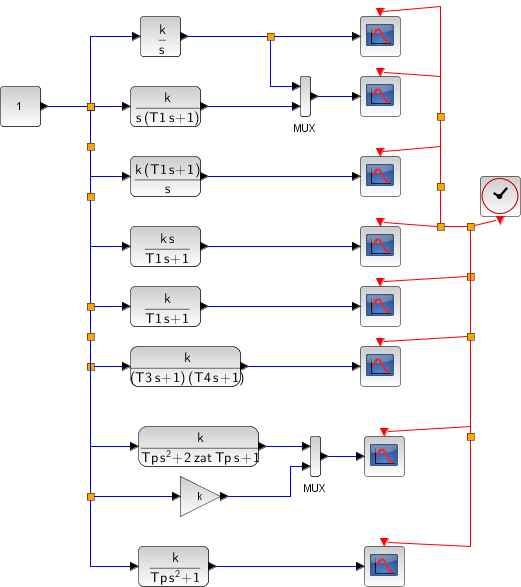
\includegraphics[width=0.6\textwidth]{sim}
	\caption{Схема моделирования типовых динамических звеньев}\label{sim}
\end{figure}


\subsection{Интегрирующее звено}
Переходной функцией интегрирующего звена является прямая, пересекающая начало координат (рис. \ref{plot_int}). Передаточная функция имеет вид $y=\dfrac{k}{s}g$. Переходную функцию $h(t)=kt$ можно описать одним лишь коэффициентом $k$, по графику видно, что он является 5.
\begin{figure}[H]
	\centering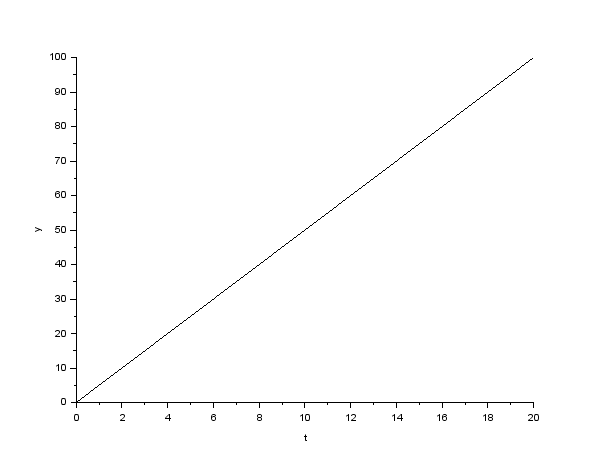
\includegraphics[width=0.6\textwidth]{plot_int.png}
	\caption{График переходной функции интегрирующего звена}\label{plot_int}
\end{figure}

\subsection{Интегрирующее звено c замедлением}
Переходной функцией интегрирующего звена с замедлением является  экспонента, стремящаяся к прямой (рис. \ref{plot_int_slow}). Передаточная функция имеет вид $y=\dfrac{k}{s(Ts+1)}g$. Переходная функция $h(t)=k(t-T(1-\exp^{-\frac{t}{T}}))$ описывается коэффициентами $T$ и $k$. Коэффициент прямой $k$, к которой стремится ветвь, равен 5; период времени замедления $T$=2
\begin{figure}[H]
	\centering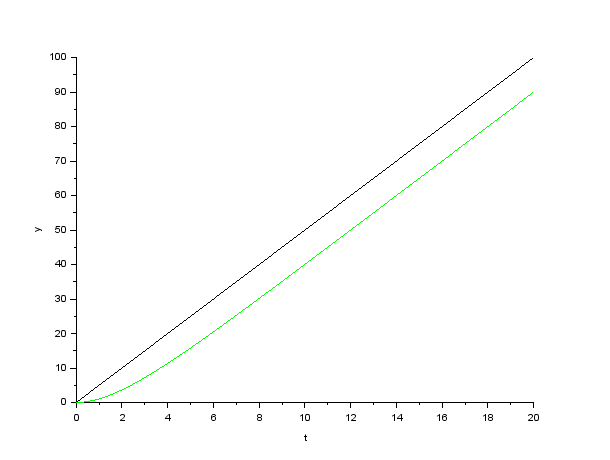
\includegraphics[width=0.6\textwidth]{plot_int_slow.png}
	\caption{График переходной функции интегрирующего звена с замедлением}\label{plot_int_slow}
\end{figure}

\subsection{Изодромное звено}
Переходной функцией изодромного звена является прямая, пересекающая ординату в точке $kT$ (рис. \ref{plot_iso}). Передаточная функция имеет вид $y=\dfrac{k(Ts+1)}{s}g$. Переходная функция $h(t)=k(t+T)$. Коэффициент усиления $k=5$ находится из наклона прямой, а $T=2$ из пересечения прямой с ординатой. 
\begin{figure}[H]
	\centering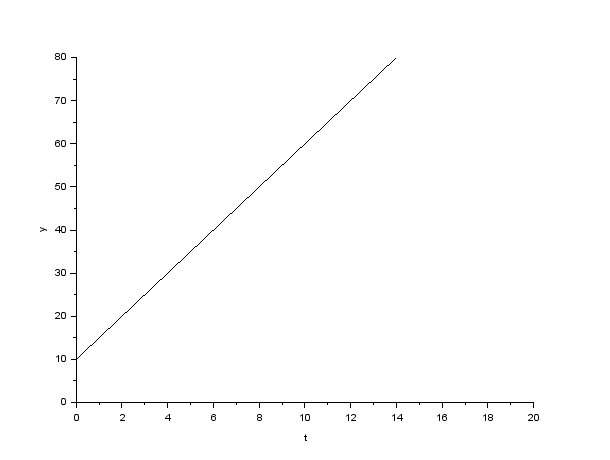
\includegraphics[width=0.6\textwidth]{plot_iso.png}
	\caption{График переходной функции изодромного звена}\label{plot_iso}
\end{figure}

\subsection{Реальное дифференцирующее звено}
Переходной функцией реального дифференцирующего звена является гипербола, пересекающая ординату в точке $k/T$ (рис. \ref{plot_dif}) и стремящуюся к нулю. Передаточная функция имеет вид $y=\dfrac{ks}{Ts+1}g$. Переходная функция $h(t)=\dfrac{k}{T}\exp^{-\frac{t}{T}}$. Проведя касательную к гиперболе в точке ее пересечения с ординатой, найдем постоянную $T=2$ в точке пересечения касательной абсциссы. $k=5$ найдем из точки пересечения графика с ординатой
\begin{figure}[H]
	\centering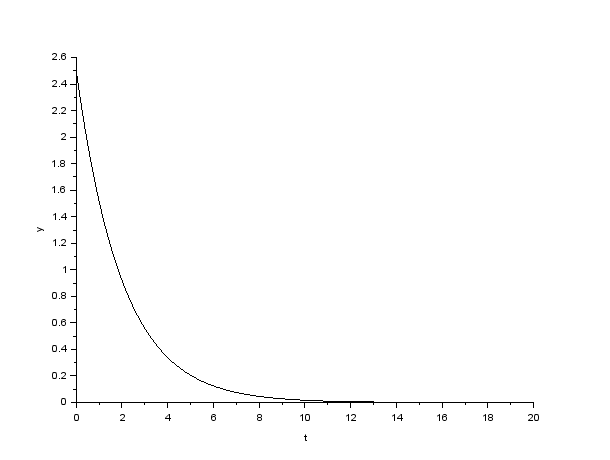
\includegraphics[width=0.6\textwidth]{plot_dif}
	\caption{График переходной функции реального дифференцирующего звена}\label{plot_dif}
\end{figure}

\subsection{Апериодическое звено 1-го порядка}
Переходной функцией апериодического звена является гипербола, пересекающая начало координат (рис. \ref{plot_ap}). Передаточная функция имеет вид $y=\dfrac{k}{Ts+1}g$. Переходная функция $h(t)=k(1-\exp^{-\frac{t}{T}})$. График функции стремится к прямой $y(t)=k$, откуда находим  $k=5$. Проведя касательную к гиперболе в начале координат, найдем постоянную $T=2$ равную абсциссе точки пересечения касательной с  $y(t)=k$.
\begin{figure}[H]
	\centering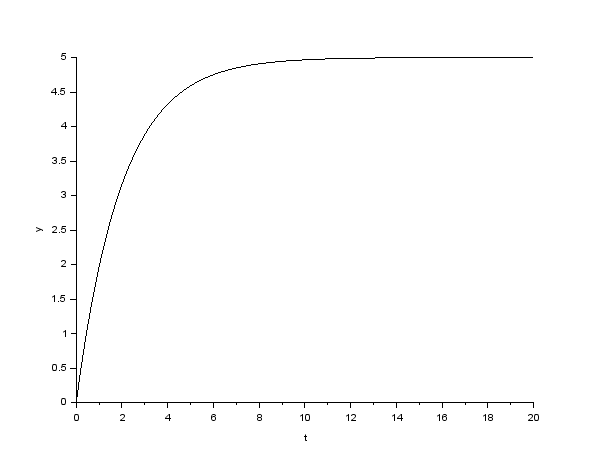
\includegraphics[width=0.6\textwidth]{plot_ap.png}
	\caption{График переходной функции апериодическое звено 1-го порядка}\label{plot_ap}
\end{figure}

\subsection{Апериодическое звено 2-го порядка}
Переходной функцией апериодического звена является гипербола, пересекающая начало координат (рис. \ref{plot_app}). Передаточная функция имеет вид $y=\dfrac{k}{T_2^2s^2+T_1s+1}g$, при условии $T_1>2T_2$ (корни знаменателя действительные и отрицательные) и записывается также $y=\dfrac{k}{(T_3s+1)(T_4s+1)}g$, переход может быть сделан $T_3=\dfrac{T_1}{2}+\sqrt{\dfrac{T_1^2}{4}-T_2^2}$ $T_4=\dfrac{T_1}{2}-\sqrt{\dfrac{T_1^2}{4}-T_2^2}$.
Переходная функция $h(t)=k(1-\dfrac{T_3}{T_3-T_4}\exp^{-\frac{t}{T_3}}+\dfrac{T_4}{T_3-T_4}\exp^{-\frac{t}{T_4}})$. График функции стремится к прямой $y(t)=k$, откуда находим  $k=5$. Проведя касательную к гиперболе, найдем пресечения касательной с абсциссой и прямой $y(t)=k$, откуда параметры $T_3=1$ и $T_3+T_4=6$ соотвественно. 
\begin{figure}[H]
	\centering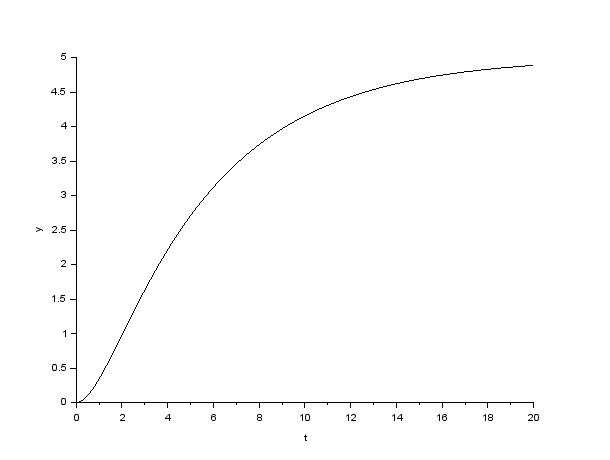
\includegraphics[width=0.6\textwidth]{plot_app.png}
	\caption{График переходной функции апериодическое звено 1-го порядка}\label{plot_app}
\end{figure}

\subsection{Колебательное звено}
Переходной функцией колебательного звена является затухающая синусоида(рис. \ref{plot_kol}). Передаточная функция имеет вид $y=\dfrac{k}{T_2^2s^2+T_1s+1}g$, при условии $T_1<2T_2$ (корни знаменателя комплексные) и записывается также $y=\dfrac{k}{T^2s^2+2\varsigma s+1}g$. 
Переходная функция $h(t)=k(1-\exp^{-\sigma t}(\cos \omega t + \dfrac{\sigma}{\omega}\sin \omega t)$, где $\sigma=\dfrac{\varsigma}{T}=\dfrac{\omega}{\pi}\ln\dfrac{a_1}{a_2}, \omega=\dfrac{1}{T}\sqrt{1-\varsigma^2}, a_1 a_2-$ амплитуды колебаний первого и второго полупериода относительно $y(t)=k$. График функции стремится к прямой $y(t)=k$, откуда находим  $k=5$ $a_1=1.56 $ $a_2=0.51 $. Найдем период колебаний равный $\dfrac{2 \pi}{\omega}$, отсюда $\omega=0.54$. 
Далее $\sigma=0.192 $ $\varsigma=\sqrt{\dfrac{1}{\dfrac{\omega^2}{\sigma^2}+1}}=0.33 $ $T=\dfrac{\varsigma}{\sigma}=1.74$
\begin{figure}[H]
	\centering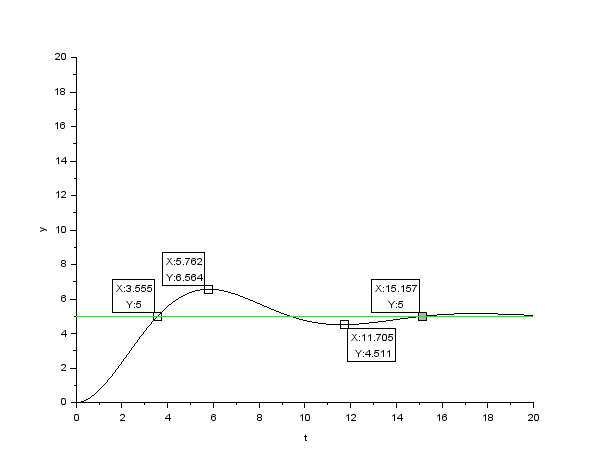
\includegraphics[width=0.6\textwidth]{plot_kol.png}
	\caption{График переходной функции колебательного звена}\label{plot_kol}
\end{figure}

\subsection{Консервативное звено}
Переходной функцией колебательного звена является незатухающая синусоида(рис. \ref{plot_con}). Передаточная функция имеет вид $y=\dfrac{k}{T^2s^2+1}g, \varsigma=0$.
Переходная функция $h(t)=k(1-\cos \omega t)$, где $omega=\dfrac{1}{T}$. Средняя линяя графика прямая $y(t)=k$, откуда $k=5$. Найдем период колебаний равный $\dfrac{2 \pi}{\omega}$, отсюда $\omega=0.58 \rightarrow T=1.73$. 
\begin{figure}[H]
	\centering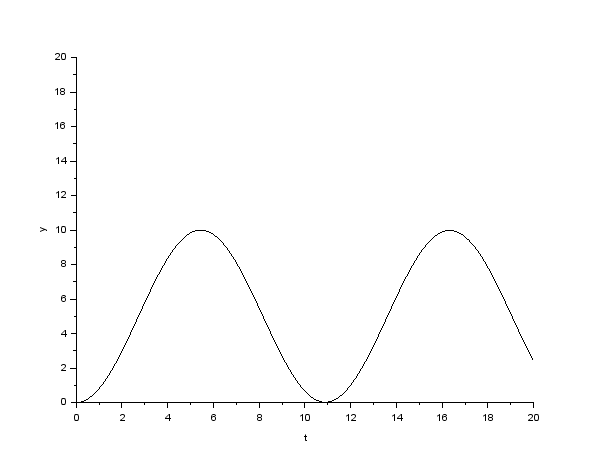
\includegraphics[width=0.6\textwidth]{plot_con.png}
	\caption{График переходной функции консервативного звена}\label{plot_con}
\end{figure}

\section{Вывод}
В ходе данной работы были успешно промоделированы типовые динамические звенья, определены параметры передаточных и переходных функций.
\end{document}